% To je predloga za poročila o domačih nalogah pri predmetih, katerih
% nosilec je Blaž Zupan. Seveda lahko tudi dodaš kakšen nov, zanimiv
% in uporaben element, ki ga v tej predlogi (še) ni. Več o LaTeX-u izveš na
% spletu, na primer na http://tobi.oetiker.ch/lshort/lshort.pdf.
%
% To predlogo lahko spremeniš v PDF dokument s pomočjo programa
% pdflatex, ki je del standardne instalacije LaTeX programov.

\documentclass[a4paper,11pt]{article}
\usepackage{a4wide}
\usepackage{fullpage}
\usepackage[utf8x]{inputenc}
\usepackage[slovene]{babel}
\selectlanguage{slovene}
\usepackage[toc,page]{appendix}
\usepackage[pdftex]{graphicx} % za slike
\usepackage{setspace}
\usepackage{color}
\definecolor{light-gray}{gray}{0.95}
\usepackage{listings} % za vključevanje kode
\usepackage{hyperref}
\renewcommand{\baselinestretch}{1.2} % za boljšo berljivost večji razmak
\renewcommand{\appendixpagename}{Priloge}

\lstset{ % nastavitve za izpis kode, sem lahko tudi kaj dodaš/spremeniš
language=Python,
basicstyle=\footnotesize,
basicstyle=\ttfamily\footnotesize\setstretch{1},
backgroundcolor=\color{light-gray},
}

\title{Naloga 1}
\author{Gašper Petelin (63140191)}
\date{\today}

\begin{document}

\maketitle


\section{Programska oprema}

\subsection{Knjižnjica in programski jezik}

Za analizo mrež je uporabljen programski jezik Python in knjižnjica NetworkX. Python je izbran zato, ker jezik omogoča hitro prototipiranje, knjižnjica NetworkX pa je ena izmed bolj dokumentiranih knjižnjic za delo z grafi.

\subsection{Karate klub}

Karate klub je sestavljen iz 34 vozlišč in 78 povezav med temi vozlišči. Slika \ref{slika1} prikazuje strukturo omrežja o povezanosti članov karate kluba. 

\begin{lstlisting}
import networkx as nx
import matplotlib.pyplot as plt

G=nx.karate_club_graph()

print("Number of nodes:", G.number_of_nodes())
print("Number of edges:", G.number_of_edges())

nx.draw(G)
plt.show()
\end{lstlisting}

\begin{figure}[htbp]
\begin{center}
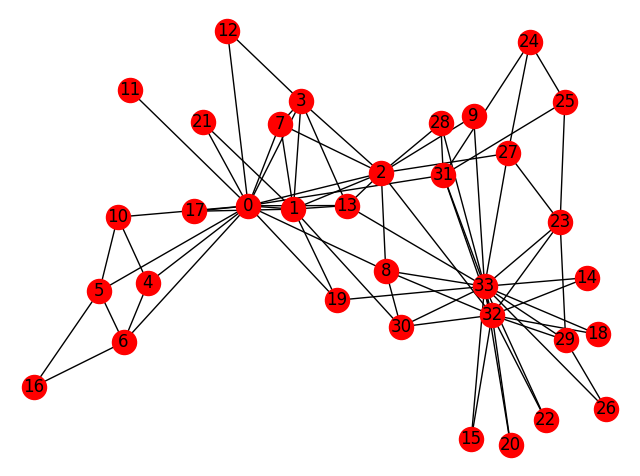
\includegraphics[scale=0.4]{karate.png}
\caption{Slika strukture omrežja članov karate kluba.}
\label{slika1}
\end{center}
\end{figure}



\section{Izbira omrežja}

\subsection{Epinions ocene produktov}

Epinions product ratings (\href{http://konect.uni-koblenz.de/networks/epinions-rating}{http://konect.uni-koblenz.de/networks/epinions-rating}) je skupek podatkov, ki predstavljajo uporabnike, produkte in ocene, ki so jih uporabniki dodelili posameznim produktom. Graf je dejansko dvodelni graf (bipartite graph), kjer je vsako vozlišče uporabnika povezano z vozlišči produktov. Vse povezave imajo določeno težo, ki predstavlja oceno in datum, kdaj je bila ocena dodeljena.

Celoten graf vsebuje 876252 vozlišč (755760 uporabnikov + 120492 izdelkov) in 13668320 povezav (ocen). Povprečna stopnja vozlišča je 31.1972.

\begin{lstlisting}
from numpy import genfromtxt
import numpy as np
import networkx as nx

data = genfromtxt("\\data\\out.epinions-rating", delimiter=' ', skip_header=1)
		 .astype(int)

users = set(data[:, 1])
products = set(data[:, 0])

G = nx.Graph()
for u in users:
    G.add_node("U"+str(u))
for p in products:
    G.add_node("P"+str(p))
for u, p in zip(data[:, 1], data[:, 0]):
    G.add_edge("U"+str(u), "P"+str(p))

print("Number of nodes:", G.number_of_nodes())
print("Number of edges:", G.number_of_edges())
print("Average degree:", np.mean([d for id,d in G.degree()]))
\end{lstlisting}

\subsection{Erdos-Renyi graf}

Za generiranje grafa je bila uporabljena funkcija, ki je že ustvarjena v paketu NetworkX, kjer podamo število vozlišč in število povezav. V tem primeru ima graf 876252 vozlišč, 13668320 povezav, povprečna stopnja vozlišča pa je 31.1972.

\begin{lstlisting}
import numpy as np
import networkx as nx

G = nx.gnm_random_graph(876252, 13668320)

print("Number of nodes:", G.number_of_nodes())
print("Number of edges:", G.number_of_edges())
print("Average degree: ", np.mean([d for id,d in G.degree()]))
\end{lstlisting}


\section{PageRank}



\subsection{Epinions ocene produktov}

Za najpomembnejše vozlišče je bilo v tem primeru izbrano vozlišče U82639. Tabela \ref{my-label2} prikazuje 10 vozlišč z največji rankom, ki ga dodeli algoritem. Števila, ki jih dobimo z algoritmom nimajo nekakšnega večjega pomena. To je vidno že iz vrednosti, ki jih dobimo, saj je prvih 10 vrednosti med seboj zelo podobnih. Nobeno izmed vozlišč ne izstopa kot preveč pomembno v primerjavi z drugimi vozlišči.

\begin{table}[]
\centering
\caption{Vozlišča grafa Epinions z največjo oceno algoritma PageRank.}
\label{my-label2}
\begin{tabular}{|l|l|lll}
\cline{1-2}
ID &  Ocena &  &  &  \\ \cline{1-2}
 
 
 U82639& 1.8785019340039697e-06&  &  &  \\ \cline{1-2}
 U105625& 1.8168748457109415e-06&  &  &  \\ \cline{1-2}
 U407122& 1.8079826377995992e-06&  &  &  \\ \cline{1-2}
 U175731& 1.7915104927271082e-06&  &  &  \\ \cline{1-2}
 U368324& 1.7839845841842157e-06&  &  &  \\ \cline{1-2}
 U61580& 1.7780805161921018e-06&  &  &  \\ \cline{1-2}
 U9260& 1.769420716877027e-06&  &  &  \\ \cline{1-2}
 U16863& 1.7659642065503108e-06&  &  &  \\ \cline{1-2}
 P1851& 1.7648999264856154e-06&  &  &  \\ \cline{1-2}
 U89528& 1.7548383835390646e-06&  &  &  \\ \cline{1-2}
\end{tabular}
\end{table}

\begin{lstlisting}
#G = Graf, ki je sestavljen z branjem datoteke (prejsnja naloga).
pr = nx.pagerank(G, alpha=0.9)

items = list(pr.items())
items.sort(key=lambda x: x[1], reverse=True)
for x,y in items[:10]:
    print(x, y)
\end{lstlisting}

\subsection{Erdos-Renyi graf}

Algoritem PageRank na grafu tipa Erdos-Renyi najbolj pomembnemu vozlišču dodeli oceno 2.156e-06
 in sicer vozlišču z število 804336.

\begin{table}[]
\centering
\caption{Vozlišča grafa Erdos-Renyi z največjo oceno algoritma PageRank.}
\label{my-label3}
\begin{tabular}{|l|l|lll}
\cline{1-2}
ID &  Ocena &  &  &  \\ \cline{1-2}
 
 
 804336& 2.156372605421521e-06&  &  &  \\ \cline{1-2}
 563952& 2.149805543078277e-06&  &  &  \\ \cline{1-2}
 79229& 2.1076087950122483e-06&  &  &  \\ \cline{1-2}
 822366& 2.0945992144791375e-06&  &  &  \\ \cline{1-2}
 727146& 2.072435694957939e-06&  &  &  \\ \cline{1-2}
 709807& 2.0573393124521594e-06&  &  &  \\ \cline{1-2}
 173284& 2.0499670044212486e-06&  &  &  \\ \cline{1-2}
 164890& 2.049064910122371e-06&  &  &  \\ \cline{1-2}
 99368& 2.0464330083141966e-06&  &  &  \\ \cline{1-2}
 613676& 2.0338221090933993e-06&  &  &  \\ \cline{1-2}
 
\end{tabular}
\end{table}

Podobno kot v prejšnjem primeru se tudi tu deset najbolje ocenjenih vozlišč med seboj ne razlikuje dovolj, da bi lahko rekli, da je katero izmed njih veliko bolj pomembno kot druga vozlišča.

\begin{lstlisting}
G = nx.gnm_random_graph(876252, 13668320)
pr = nx.pagerank(G, alpha=0.9)

items = list(pr.items())
items.sort(key=lambda x: x[1], reverse=True)
for x,y in items[:10]:
    print(x, y)
\end{lstlisting}


\end{document}
